\section{5-28 notes}
\subsection{New parameterization}
I found a parameterization of the beta distribution, where you specify the \emph{mode} and a dispersion parameter.  If the dispersion parameter is between 0 and 1, then the distribution is guaranteed to be unimodal.

\subsection{Simple model used for analysis}
I tried to analyze the cause of bias using the simplest model below:

This is basically the part of the model that predicts $a$.

\begin{eqnarray}
f^a(x) &=& \frac{1}{1+e^{-x}} \\
\mu_i^a &=& f^a(\mu_{pop}^a + Bx_i) \\
a_i &\sim& Beta(\mu_i^a, \phi^a) \\
B &\sim& U(-\infty,\infty)
\end{eqnarray}

\subsection{Plots}
\begin{enumerate}

\item First question is whether we should have a linear model for the mean or mode of the beta distribution that $a$ comes from.  That is, should $\mu_i^a$ be the mean or mode of a beta distribution?  In Figure 1, in each subplot, I plot several beta distributions.  All of them have the same \emph{mean}, but different $\phi$'s.  
\begin{figure}
\begin{center}
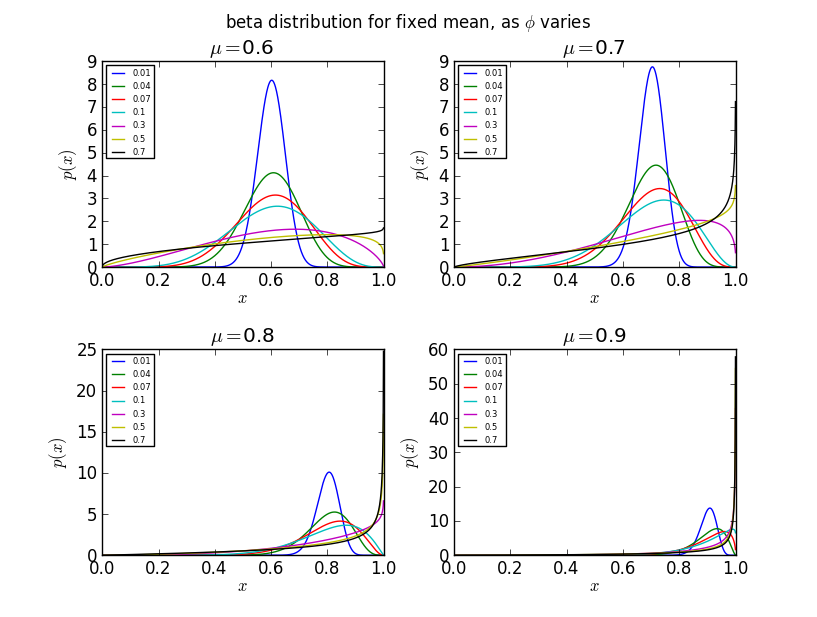
\includegraphics[width=4in, height=3in]{/Users/glareprotector/prostate_git/glare/tex_files/sections/analyze_bias/files/beta_vs_mu.png}
\caption{}
\end{center}
\end{figure}


\item In Figure 2, in each subplot, I plot several beta distributions.  All of them have the same \emph{mode}, but different $\phi$.  It seems better to have a linear model for the mode of beta distributions 
\begin{figure}
\begin{center}
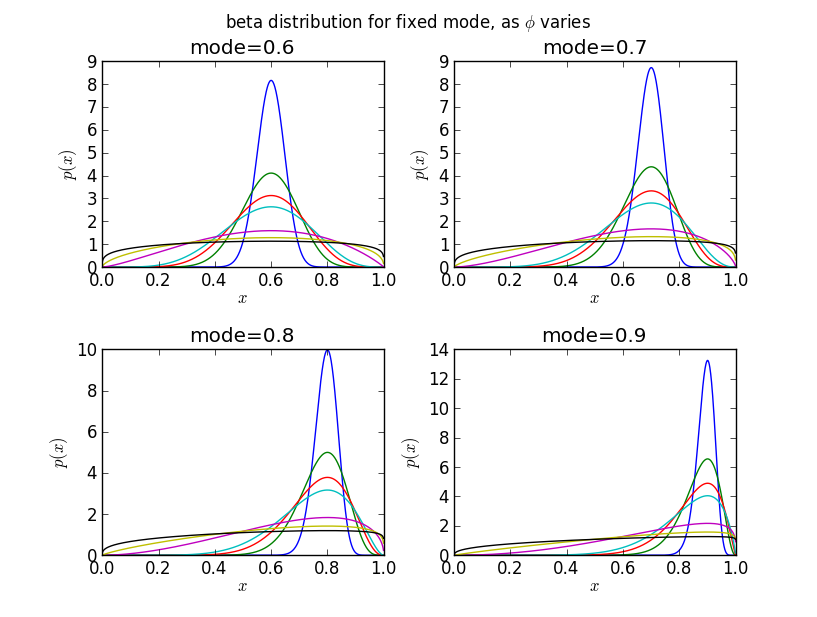
\includegraphics[width=4in, height=3in]{/Users/glareprotector/prostate_git/glare/tex_files/sections/analyze_bias/files/beta_vs_mode.png}
\caption{}
\end{center}
\end{figure}

\item Let's try to get a grasp on the $\phi$ parameter.  In Figure 3, in each subplot, I fix $\phi$ and plot a beta distribution with various modes, with that $\phi$.
\begin{figure}
\begin{center}
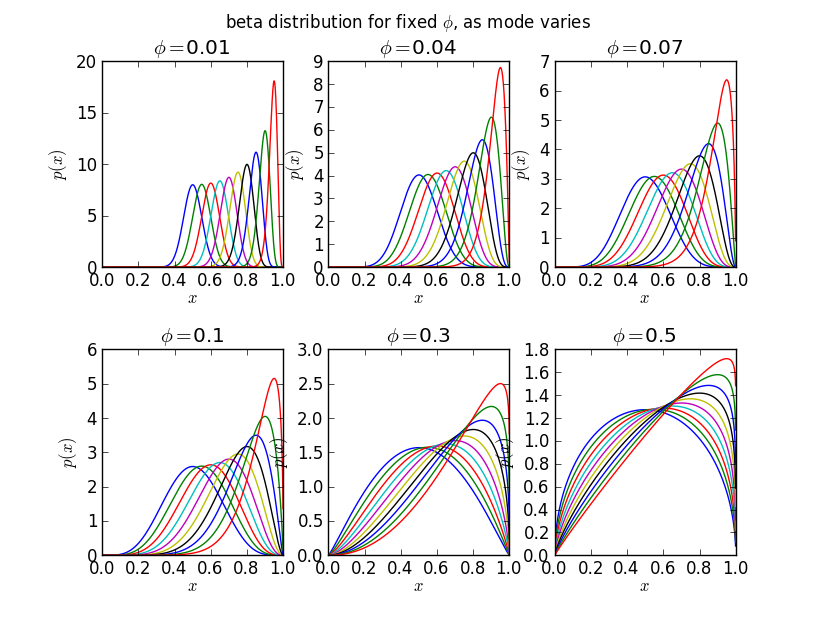
\includegraphics[width=4in, height=3in]{/Users/glareprotector/prostate_git/glare/tex_files/sections/analyze_bias/files/beta_phi.png}
\caption{}
\end{center}
\end{figure}

\item Now, goal is to see if this beta regression produces biased MLE estimates of B.  In Figure 4, I set B=1.0.  Below, for each $(\mu_{pop}^a,\phi)$ combination, I do the following: 
    \begin{enumerate}
    \item let $X_i$ be number between -1 and 1.  The $X_1, \ldots X_n$ are chosen to be equally spaced between -1 and 1.  $n=100$.
    \item for each $X_i$, generate $a_i$ according to the model, with randomness.$(\mu_{pop}^a$ and $\phi^a)$ and B are all specified, so this is well defined.  
    \item Plot the distribution of $P(B;X_i,a_i,\phi,\mu_{pop}^a)$  
    \end{enumerate}
These plots are mildly informative.  Small $\phi$'s get rid of bias.  It's not clear if higher $\phi$ leads to bias in one direction.    

\begin{figure}
\begin{center}
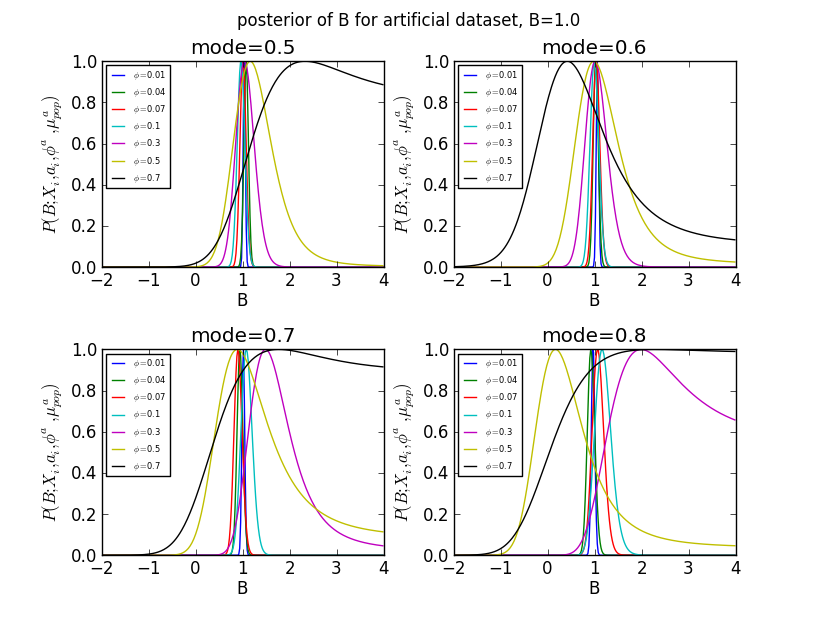
\includegraphics[width=4in, height=3in]{/Users/glareprotector/prostate_git/glare/tex_files/sections/analyze_bias/files/B_posterior.png}
\caption{}
\end{center}
\end{figure}

\item Try to figure out the cause of the bias.  In Figure 5, I fix x. I plot P(x;mode,$\phi$), assuming $x \sim Beta(mode,\phi)$.  Note that for high values of, x the mode of $P(x;mode,\phi)$ does not occur at $x$.  I do this for 4 values of x.

\begin{figure}
\begin{center}
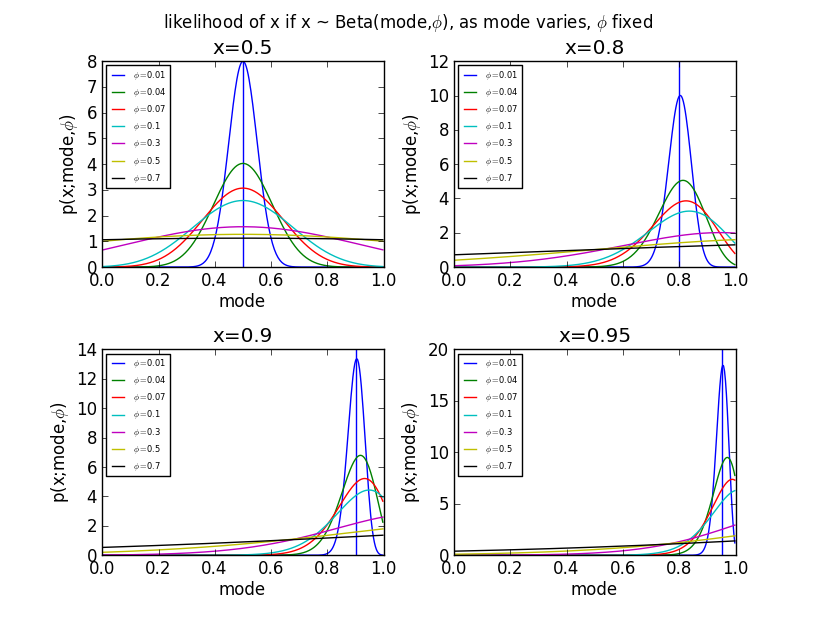
\includegraphics[width=4in, height=3in]{/Users/glareprotector/prostate_git/glare/tex_files/sections/analyze_bias/files/infer_beta_mode.png}
\caption{}
\end{center}
\end{figure}

\item From previous plot, we know that if x is close to 1, and we assume x ~ Beta(mode,$\phi$), the MLE estimate of mode will be biased.  Let's see how this causes the estimate of B to be biased.  In Figure 6, I basically repeat the previous plots where I simulated data and tried to infer B.  However, here there is only 1 datapoint, $x_0=1$, and I let $a_0=\mu_0^a$.

\begin{figure}
\begin{center}
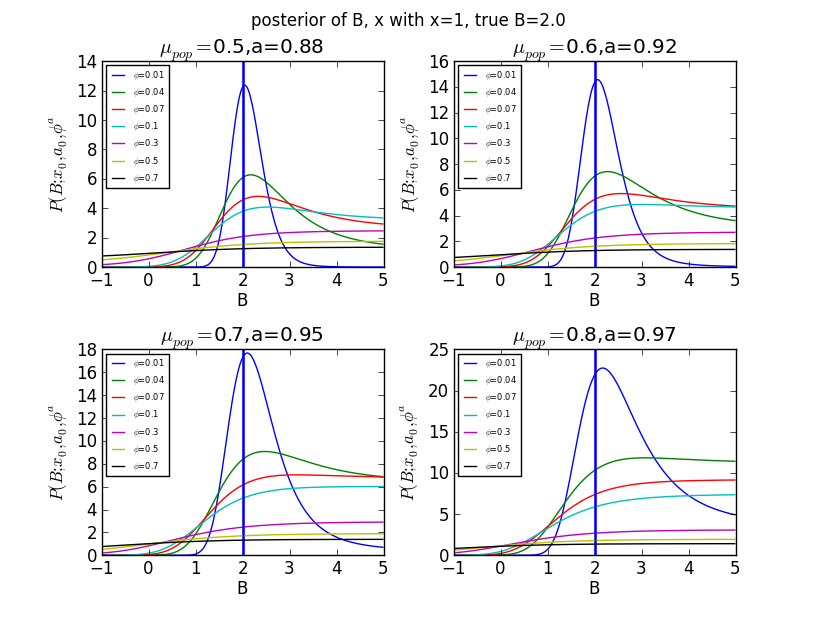
\includegraphics[width=4in, height=3in]{/Users/glareprotector/prostate_git/glare/tex_files/sections/analyze_bias/files/B_posterior_simple.png}
\caption{}
\end{center}
\end{figure}

\end{enumerate}